En este punto, se nos asignó la tarea de implementación de un scheduler Round-Robin que no permita la migración de procesos
entre núcleos. La asignación de CPU se realizaría en el momento de carga de un proceso y el núcleo correspondiente al mismo sería aquel con menor cantidad de procesos activos totales.

\bigskip

\textbf{Implementación}

La implementación de este scheduler no difiere mucho del de la del ejercicio 4, sólo que en este caso se tiene una cola de procesos por CPU. Además, se posee un entero por CPU (en un vector) que indica la cantidad de procesos activos para cada uno de estos, a ser utilizados cuando se cargue un proceso nuevo. Por último, poseemos un mapa de procesos para saber a qué CPU corresponde cada uno.

Al cargar un proceso, se obtiene el índice (CPU) del mínimo elemento del vector de \"activos\" y con eso se empuja el proceso a la cola correspondiente y se aumenta la cantidad de activos. Por último, se agrega el proceso con su CPU al mapa de procesos.

Al hacer un tick, la única diferencia con el código del ejercicio 4, además de elegir la cola correspondiente al cpu indicado, es al momento de finalización de una tarea. En este caso, se le resta uno a la cantidad de activos del CPU y se elimina al proceso del mapa de procesos. Luego, es análogo.

Al desbloquearse un proceso, simplemente se obtiene el CPU del mismo a través del mapa de procesos. Con esto, se empuja al proceso al core correspondiente.

\bigskip

\textbf{Ejemplo 1}

Un escenario en el que este scheduler es peor en contraposición con el Round-Robin tradicional, es cuando se van alternando procesos de corta duración con procesos que tarden bastante, como por ejemplo sería el caso de dos c\'alculos que difieran mucho en complejidad. Imaginemos el siguiente caso. Somos la central que controla los subtes de una mediana ciudad. Por una falta de previsi\'on en el dise\~no del sistema de subterraneos, hay ocasiones en que los subtes quedan ubicados de forma tal que es inviable su correcto funcionamiento. Por suerte, el sistema logra anticipar este escenario, a partir de lo cu\'al debe estimar el tiempo que demandar\'a la soluci\'on, por un lado, y definir la correcta sucesi\'on de movimientos que tiene que hacer cada unidad para evitar el colapso. En este caso, terminarían primero los procesos de corta duración, quedando CPUs sin ningún proceso asignado; no se estarían utilizando, realentizando el tiempo de compleción de los procesos y probablemente su tiempo de espera. Sin embargo, la latencia no se vería afectada y sería la misma en ambos casos.

Para ejemplificar esto, construimos un lote de 7 tareas "TaskCPU", alternadas en tiempos de 1 y 8 ciclos. A continuación, se presenta un gráfico de tal lote que simula la situación planteada:

\begin{figure}[h]
    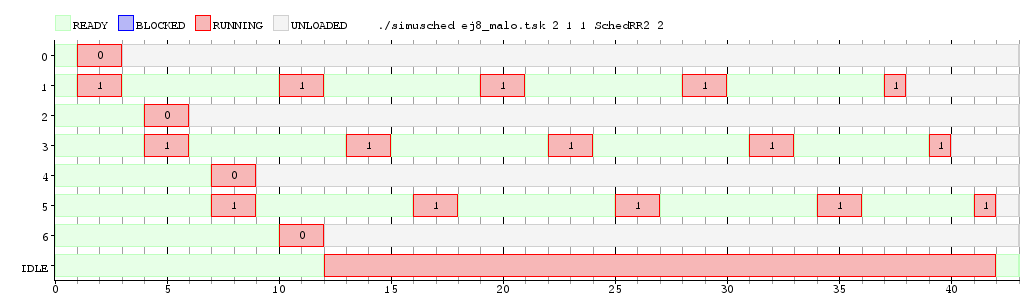
\includegraphics[width=1\textwidth]{ej8MaloRR2}
    \caption{Ejecución en Round-Robin 2}
    \label{RR2Malo}
\end{figure}

Como se muestra en la figura \ref{RR2Malo}, podemos notar lo antes mencionado. Con este nuevo scheduler, a partir del instante 16, el CPU 0, ya no posee ninguna tarea a ejecutar, siendo que terminaron todas las que fueron asignadas al mismo al momento de carga. Por lo tanto, queda en IDLE, mientras que el CPU 1 ejecuta alternadamente los 3 procesos restantes.

En la siguiente tabla mostramos distintas métricas, correspondientes a esta simulación:
% Tabla RR2
\begin{table}[h]
  \caption{Ejecución en Round-Robin 2}
  \centering
    \begin{tabular}{c c c c c}
    \hline
          & Latencia & Espera & Compleción & Ratio (E/C) \\
    \hline
        0 &     1    &    1   &      3     &     0.333   \\
        1 &     1    &   29   &     38     &     0,763   \\
        2 &     4    &    4   &      6     &     0.666   \\
        3 &     4    &   31   &     40     &     0.775   \\
        4 &     7    &    7   &      9     &     0.777   \\
        5 &     7    &   33   &     42     &     0,785   \\
        6 &     10   &   10   &     12     &     0.833   \\
        AVG & 4,857  & 16,428 &   21,428   &     0,705   \\
    \end{tabular}
\end{table}


En cambio, en la figura \ref{RRMalo} (que se presenta a continuación), podemos observar, como con el Round-Robin tradicional, cuando terminan de ejecutarse las tareas cortas (0, 2, 4 y 6), el CPU 1 sigue siendo utilizado por las restantes. Notar que aunque perdemos 1 ciclo extra por cada cambio de CPU, los procesos siguen terminando antes que con el nuevo scheduler implementado.

\begin{figure}[h]
    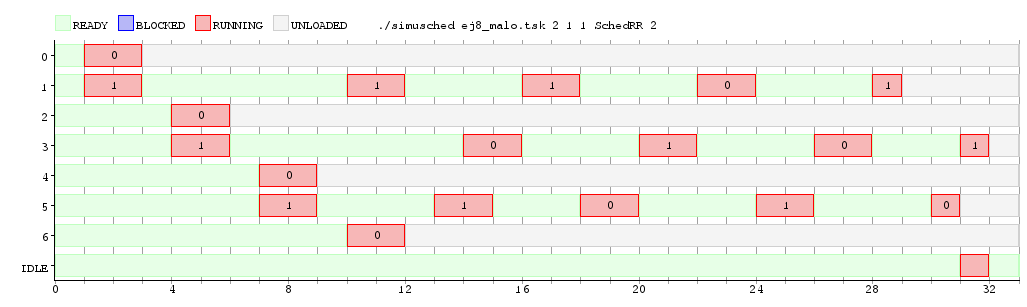
\includegraphics[width=1\textwidth]{ej8MaloRR}
    \caption{Ejecución en Round-Robin Tradicional}
    \label{RRMalo}
\end{figure}

En la siguiente tabla volcamos datos con las mismas métricas que en la tabla correspondiente a \textit{Round-Robin 2}.

% Tabla RR1
\begin{table}[h]
  %\captionsetup{justification=justified,singlelinecheck=false}
  \caption{Ejecución en Round-Robin Tradicional}
  \centering
    \begin{tabular}{c c c c c}
    \hline
          & Latencia & Espera & Compleción & Ratio (E/C) \\
    \hline
        0 &     1    &    1   &      3     &    0.333    \\
        1 &     1    &   20   &     29     &    0,690    \\
        2 &     4    &    4   &      6     &    0.666    \\
        3 &     4    &   23   &     32     &    0,719    \\
        4 &     7    &    7   &      9     &    0.777    \\
        5 &     7    &   22   &     31     &    0,710    \\
        6 &     10   &   10   &     12     &    0.833    \\
        AVG & 4,857  & 12,429 &   17,428   &    0,675    \\
    \end{tabular}
\end{table}

Como supusimos anteriormente, podemos ver como el tiempo de espera y compleción de los procesos largos es menor en \textit{Round-Robin Tradicional}, por lo que en promedio también es mejor. La latencia se mantiene estable.

\bigskip

\textbf{Ejemplo 2}

Sin embargo, este nuevo tipo de scheduler resulta útil en algunas situaciones. Tal es el caso cuando se quisiera lanzar un proceso que ejecute en tiempo real. A modo ilustrativo, en el ejemplo anterior, podría el usuario querer ejecutar alguna especie de simulación. Imaginemos que ya se terminaron de ejecutar los procesos cortos y queda un core libre. Entonces, la simulación correría sin interrupciones, y aunque llegaran más procesos, en principio caerían probablemente  en el mismo CPU (si los otros procesos no terminaron), pero estaría balanceado. El tiempo de espera sería menor, como probablemente también la latencia de la simulación.

Para reflejar este comportamiento, modificamos el lote de tareas anterior, agregando la tarea 7 (TaskCPU de 12 ciclos) en el momento 4. Además, agregamos dos tareas pequeñas más que interrumpen a la tarea 7. El gráfico correspondiente se encuentra a continuación:

\begin{figure}[h]
    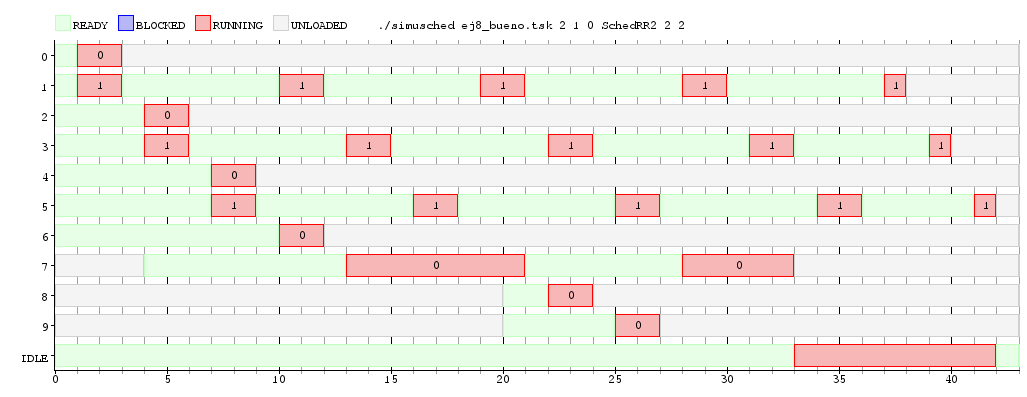
\includegraphics[width=1\textwidth]{ej8BuenoRR2}
    \caption{Ejecución en Round-Robin 2}
    \label{RR2Bueno}
\end{figure}

Como mencionamos, si bien la tarea 7 es interrumpida, tiene un corto tiempo de espera (7 ciclos). Compararlo con la figura \ref{RR2Malo} que se presenta a continuación:

\begin{figure}[h]
    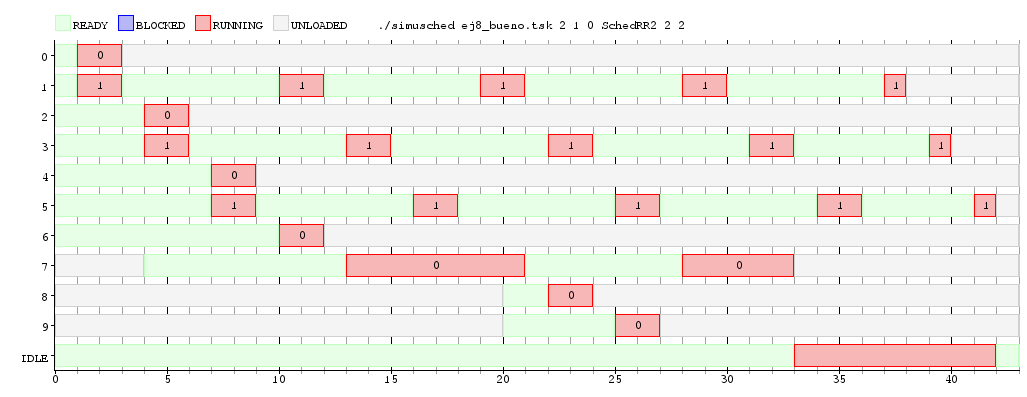
\includegraphics[width=1\textwidth]{ej8BuenoRR2}
    \caption{Ejecución en Round-Robin Tradicional}
    \label{RR2Malo}
\end{figure}

Si bien la tarea 7 tiene la misma latencia en ambos casos, el tiempo de espera es mucho mayor en el \textit{Round-Robin Tradicional}. Como sólo nos importa esta tarea realmente, presentamos una tabla comparativa entre ambos Schedulers para la tarea 7.

\begin{table}[h]
  \caption{Comparación entre schedulers para la tarea 7}
  \centering
    \begin{tabular}{c c c c c}
    \hline
            & Latencia & Espera & Compleción & Ratio (E/C) \\
    \hline
        RR  &     1    &   15   &     28     &    0.536    \\
        RR2 &     1    &    7   &     20     &    0.35     \\
    \end{tabular}
\end{table}

Notar que si no existieran las tareas 8 y 9 que interrumpen ó si hubiera un core libre, la espera sería 0. Igualmente, es notable la mejora que provee el nuevo scheduler en esta situación particular.

Además de esto, en la realidad hay otros factores a considerar que no podrían ser medidos con la simulación utilizada. Por ejemplo, en arquitecturas SMP, es importante mantener cierta afinidad al procesador asignado al proceso, para aprovechar la caché. Si hubiera cambio de procesador, el proceso llegaría con la caché vacía, produciéndose un miss y teniendo que ir a buscar los datos a memoria principal. A esto se le suma el tiempo de los cambios de procesador y de contexto que no son despreciables. En ese sentido, el nuevo scheduler sería preferible al \textit{Round-Robin Tradicional}.
